\section{Experimental Results}
\label{sec:implementation}
In order to verify the results of this work, we implemented stages 1 and 2 of the BKW algorithm. Our implementation considers LWE with short secrets but we ignore the transformation cost to produce samples with a short secret. Also, our implementation supports arbitrary bit-width windows $b$, not only multiplies of $\lceil \log_2(q)\rceil$. However, due to the fact that our implementation does not use a balanced representation of finite field elements internally -- which simplifies dealing with arbitrary bit-width windows -- our implementation does not \emph{fully} implement the half-table improvement. That is, for simplicity, our implementation only uses the additive inverse of a vector if this is trivially compatible with our internal data representation. Furthermore, our implementation does not bit-pack finite field elements. Elements always take up 16 bits of storage. Overall, the memory consumption of our implementation in stage 1 is worse by a factor of up to four compared to the estimates given in this work and the computational work in stage is worse by a factor of up to two. Finally, since our implementation is not optimised we do not report CPU times.

With these considerations in mind, our estimates are confirmed by our implementation. For example, consider Regev's parameters for $n=25$ and $t=2.3$ and $d=1$, By Lemma~\ref{lem:m} picking $m=2^{12.82}$ will result in a success probability of $\mathrm{p}_{success} \approx 0.99959$ per component and $\mathrm{P}_{success} \approx 0.99$ overall. Lemma~\ref{lem:firststep} estimates a computational cost of $2^{30.54}$ ring operation and $2^{24.19}$ calls to $\Ldis$ in stage 1. We ran our implementation with $m = \lceil 2^{12.82} \rfloor$ and window bitsize $w = 22 = \frac{n\log_2(q)}{2.3\log_2(n)}$. It required $2^{29.74}$ ring operations and $2^{23.31}$ calls to $\Ldis$ to recover one component of $\svec$. From this we conclude that Theorem~\ref{theorem:complexity1} is reasonably tight.

To test the accuracy of Lemma~\ref{lem:m} we ran our implementation with the parameters $n=25$, $q=631$, $\alpha \cdot q = 5.85$, $w = 24 = \frac{n\log_2(q)}{2.1\log_2(n)}$ and $m=2^7$. Lemma~\ref{lem:m} predicts a success rate of 53\%. In 1000 experiments we 665 times rank zero for the correct key component, while Lemma~\ref{lem:m} predicted $530$. Hence, it seems our predictions are slightly pessimistic. The distribution of the ranks of the correct component of $\svec$ in 1000 experiments is plotted in Figure~\ref{fig:ranks}.

\begin{figure}[!htb]
\centering
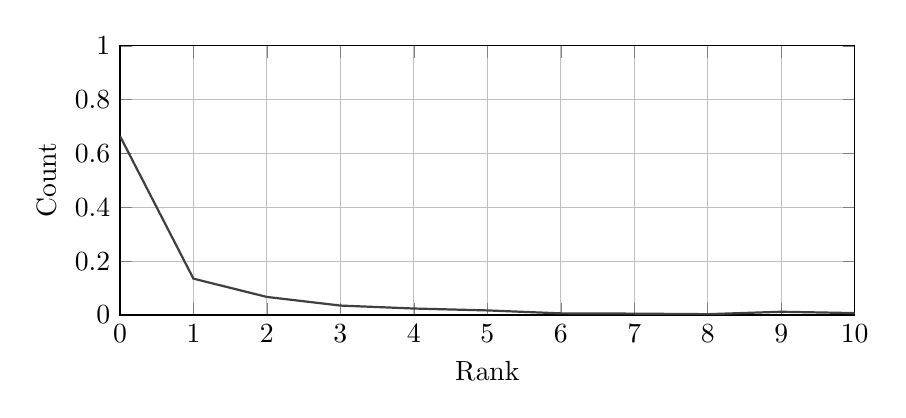
\begin{tikzpicture}[xscale=1,yscale=1]
\begin{axis}[xmin=0,xmax=10,ymin=0.0,ymax=1.00,no markers,grid=both,xlabel=Rank,ylabel=Count,width=0.9\textwidth,height=5cm]
\addplot[color=darkgray,thick] coordinates {(0, 0.665) (1, 0.135) (2, 0.067) (3, 0.035) (4, 0.024) (5, 0.017) (6, 0.006) (7, 0.005) (8, 0.003) (9, 0.012) (10, 0.007) (11, 0.006) (12, 0.003) (13, 0.004) (14, 0.002) (15, 0.0) (16, 0.002) (17, 0.002) (18, 0.0) (19, 0.0) (20, 0.0) (21, 0.001) (22, 0.002) (23, 0.0) (24, 0.0) (25, 0.0) (26, 0.0) (27, 0.0) (28, 0.0) (29, 0.0) (30, 0.0) (31, 0.0) (32, 0.0) (33, 0.0) (34, 0.001) (35, 0.0) (36, 0.0) (37, 0.0) (38, 0.0) (39, 0.0) (40, 0.0) (41, 0.0) (42, 0.0) (43, 0.0) (44, 0.0) (45, 0.0) (46, 0.0) (47, 0.0) (48, 0.0) (49, 0.0) (50, 0.001)};
\end{axis}
\end{tikzpicture}
\caption{Distribution of right key component ranks for 1000 experiments on $n=25$, $t=2.3$, $d=1$, $\mathrm{p}_{success}=0.99$.}
\label{fig:ranks}
\end{figure}

\anonymous{Our implementation will be made available soon.}{Our implementation is available at \url{http://bitbucket.org/malb/bkw-lwe}.}


